\documentclass[aspectratio=169,11pt]{beamer}
\usetheme{default}
\usecolortheme{default}
\setbeamertemplate{navigation symbols}{}
\setbeamertemplate{footline}[frame number]
\usepackage{booktabs}
\usepackage{amsmath,amssymb}
\usepackage{graphicx}
\usepackage{tikz}
\usetikzlibrary{positioning,arrows.meta,calc}
\definecolor{clr}{HTML}{2A78D6}
\definecolor{warn}{HTML}{C0392B}
\setbeamercolor{frametitle}{fg=clr}
\setbeamercolor{title}{fg=clr}
\setbeamercolor{structure}{fg=clr}
\newcommand{\Dhat}{\widehat{\Delta}}
\newcommand{\se}{\mathrm{se}}

\title{Learning How Wrong Offline Estimates Are}
\subtitle{Reliable Launch Decisions for Recommender Systems}
\author{Nihar Sagar G}
\institute{EECE, IIT Dharwad \\ PRML Course Project}
\date{10 November 2026}

\begin{document}

\begin{frame}
\titlepage
\end{frame}

\begin{frame}{The problem}
\begin{itemize}
  \item A shopping app wants to replace its recommender (the model that picks which products to show).
  \item Testing on real users (A/B test) is slow and risky.
  \item So it first \textbf{estimates offline}, from old click logs, how the new recommender would have done.
  \item Estimates have errors, so it launches only if
  \[ \text{estimated improvement} - \text{safety margin} > 0 \]
\end{itemize}
\vspace{0.5em}
\begin{block}{Question}
Is the usual safety margin big enough? \textbf{On real data: no.} It is about half as big as it should be.
\end{block}
\end{frame}

\begin{frame}{The idea in one picture: the friend who is always late}
\begin{itemize}
  \item Your friend says ``10 minutes''.
  \item Looking at the last 20 times, they arrived up to \textbf{25 minutes} late.
  \item So you plan for 25 minutes. You do not need to know \emph{why} they are late.
\end{itemize}
\vspace{0.8em}
\textbf{Our method does the same for estimates:}
\begin{itemize}
  \item Look at past decisions where we know both the offline estimate and the real result.
  \item Measure how wrong the estimates actually were.
  \item Set the safety margin from that track record.
\end{itemize}
\vspace{0.5em}
\textbf{Conformal prediction} is the statistically correct way to pick the number, so that it is right 95\% of the time.
\end{frame}

\begin{frame}{The method at a glance}
\centering
\resizebox{!}{0.68\textheight}{% Method overview, shared by the paper and the slides. Requires tikz with
% positioning, arrows.meta and calc.
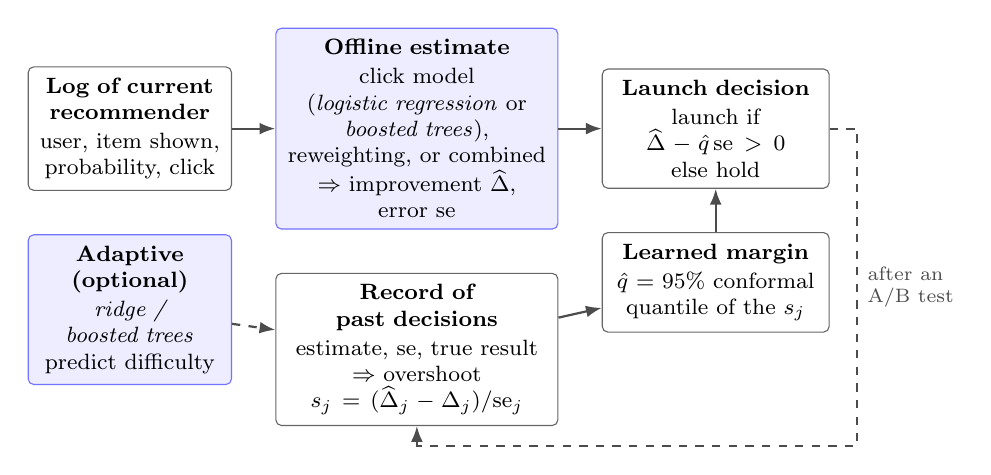
\begin{tikzpicture}[
  font=\footnotesize,
  box/.style={draw=black!60, rounded corners=2pt, align=center, inner sep=4pt, text width=#1},
  box/.default=2.6cm,
  ml/.style={box=#1, fill=blue!7, draw=blue!55},
  ml/.default=2.6cm,
  arr/.style={-{Latex[length=2mm]}, thick, black!70},
  node distance=0.45cm and 0.55cm]

\node[box=2.3cm] (log) {\textbf{Log of current\\recommender}\\[1pt]user, item shown,\\probability, click};
\node[ml=3.3cm, right=of log] (est) {\textbf{Offline estimate}\\[1pt]click model\\(\emph{logistic regression} or\\\emph{boosted trees}),\\reweighting, or combined\\[1pt]$\Rightarrow$ improvement $\widehat\Delta$,\\error $\mathrm{se}$};
\node[box=2.6cm, right=of est] (dec) {\textbf{Launch decision}\\[1pt]launch if\\$\widehat\Delta - \hat q\,\mathrm{se} > 0$\\else hold};

\node[box=3.3cm, below=0.55cm of est] (hist) {\textbf{Record of past decisions}\\[1pt]estimate, se, true result\\$\Rightarrow$ overshoot\\$s_j=(\widehat\Delta_j-\Delta_j)/\mathrm{se}_j$};
\node[box=2.6cm, below=0.55cm of dec] (q) {\textbf{Learned margin}\\[1pt]$\hat q$ = 95\% conformal\\quantile of the $s_j$};
\node[ml=2.3cm, below=0.55cm of log] (diff) {\textbf{Adaptive (optional)}\\[1pt]\emph{ridge / boosted trees}\\predict difficulty};

\draw[arr] (log) -- (est);
\draw[arr] (est) -- (dec);
\draw[arr] (hist) -- (q);
\draw[arr] (q) -- (dec);
\draw[arr, dashed] (diff) -- (hist);
\draw[arr, dashed] (dec.east) -- ++(0.35,0) |- node[pos=0.25, right, align=left, font=\scriptsize] {after an\\A/B test} ($(hist.south)+(0,-0.25)$) -- (hist.south);
\end{tikzpicture}
}
\vspace{0.5em}

\raggedright
Blue boxes contain the machine-learning models. The dashed arrow: every A/B test adds one more past decision, so the margin keeps learning.
\end{frame}

\begin{frame}{Step 1: estimating a new recommender offline}
Log of the current recommender: user $x$, item shown $a$, probability it was shown $p$, click $r$.
\vspace{0.3em}
\begin{enumerate}
  \item \textbf{Click model}: train a classifier for $P(\text{click}\mid \text{user},\text{item})$ (\textbf{logistic regression} or \textbf{gradient-boosted trees}); average its predictions over what the new recommender would show.
  \item \textbf{Reweighting}: count logged clicks, weighting items the new recommender likes more:
  $\quad w = \dfrac{P_{\text{new}}(\text{item})}{P_{\text{old}}(\text{item})}$, \quad estimate $=$ average of $w \cdot r$.
  \item \textbf{Combined}: click model, plus reweighting of its mistakes.
\end{enumerate}
\vspace{0.3em}
Improvement estimate $\Dhat$ = new click rate $-$ old click rate, with standard error $\se$.\\
All written from scratch; match the \texttt{obp} reference library to $10^{-9}$.
\end{frame}

\begin{frame}{Step 2: the learned margin}
\textbf{Usual rule:} launch if $\Dhat - 1.645\,\se > 0$.\\[0.6em]
\textbf{Our rule:}
\begin{enumerate}
  \item For each past decision $j$: how many standard errors did the estimate overshoot?
  \[ s_j = \frac{\Dhat_j - \Delta_j^{\text{true}}}{\se_j} \]
  \item Sort them; take $\hat q$ = the value that 95\% of them are below.
  \item Launch if $\Dhat - \hat q\,\se > 0$.
\end{enumerate}
If estimates were honest, $\hat q \approx 1.645$. On real data, $\hat q \approx 2.7$.
\begin{block}{Guarantee}
If the new decision is like the past ones, the margin is big enough at least 95\% of the time, \emph{even if the estimator is biased}.
\end{block}
\end{frame}

\begin{frame}{Why 1.645 is too small: the real record}
\begin{columns}[c]
\begin{column}{0.6\textwidth}
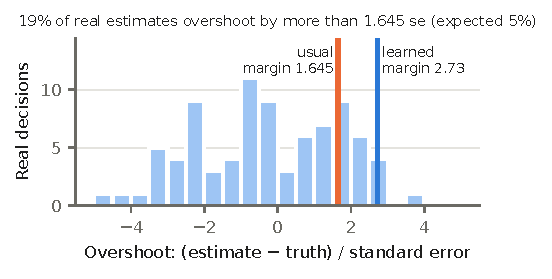
\includegraphics[width=\textwidth]{figures/error_histogram.pdf}
\end{column}
\begin{column}{0.4\textwidth}
\begin{itemize}
  \item Each bar: real decisions, by how many standard errors the estimate overshot the truth.
  \item Usual margin assumes only 5\% beyond 1.645.
  \item Real: \textcolor{warn}{\textbf{19\%}} beyond it.
  \item Learned margin \textcolor{clr}{\textbf{2.73}}: 5\% beyond.
\end{itemize}
\end{column}
\end{columns}
\end{frame}

\begin{frame}{Why the guarantee holds}
\begin{itemize}
  \item The margin is big enough exactly when $s_{\text{new}} \le \hat q$.
  \item If the new decision is like the past ones, $s_{\text{new}}$ is equally likely to land anywhere in the sorted list of $m+1$ scores.
  \item We picked $\hat q$ so that at most 5\% of positions are above it.
  \item So the margin fails at most 5\% of the time.
\end{itemize}
\vspace{0.5em}
\textbf{Assumes:} new decisions resemble past ones. \textbf{Does not assume:} unbiased estimator, correct click model, normal errors.
\end{frame}

\begin{frame}{Data}
\begin{columns}[T]
\begin{column}{0.5\textwidth}
\textbf{Real: Open Bandit Dataset}
\begin{itemize}
  \item 26M recommendations, fashion e-commerce site, 7 days, 3 campaigns
  \item Two recommenders ran \emph{at the same time} on split traffic: one random, one adaptive
  \item So each one's real click rate is the \textbf{true answer} when estimating it from the other's log
  \item 12-hour windows $\Rightarrow$ \textbf{84 real decisions}
\end{itemize}
\end{column}
\begin{column}{0.5\textwidth}
\textbf{Controlled: 6 classification datasets}
\begin{itemize}
  \item Classes $=$ items; click if the right class is shown
  \item True click rate of every recommender is exact
  \item New recommenders: retrained, naive Bayes, $k$-NN, random forest, \ldots
  \item Population shift created with \textbf{PCA}
  \item \textbf{2,688 decisions}, 27\% not better
\end{itemize}
\end{column}
\end{columns}
\end{frame}

\begin{frame}{Finding 1: real estimates are about 2$\times$ more wrong than they say}
\centering
\small
\begin{tabular}{lrrr}
\toprule
& \multicolumn{3}{c}{Actual error / reported error (1.0 = honest)}\\
\cmidrule(lr){2-4}
Estimator & usual se & grouped by page & \textbf{grouped by hour}\\
\midrule
Click model (GBT) & \textcolor{warn}{2.62} & \textcolor{warn}{2.41} & \textcolor{warn}{1.99}\\
Reweighting & \textcolor{warn}{1.67} & \textcolor{warn}{1.62} & 1.22\\
Combined (GBT) & \textcolor{warn}{1.80} & \textcolor{warn}{1.76} & 1.13\\
\bottomrule
\end{tabular}
\normalsize
\raggedright
\begin{itemize}
  \item The usual 95\% margin is big enough only \textbf{60--80\%} of the time.
  \item Grouping the 3 items on one page: no change $\Rightarrow$ not the cause.
  \item Grouping by hour: explains most of it $\Rightarrow$ \textbf{user behaviour drifts hour to hour}.
  \item Click models stay at $\sim$2: their error is \textbf{bias} from an imperfect classifier.
\end{itemize}
\end{frame}

\begin{frame}{Why: user behaviour drifts hour to hour}
\centering
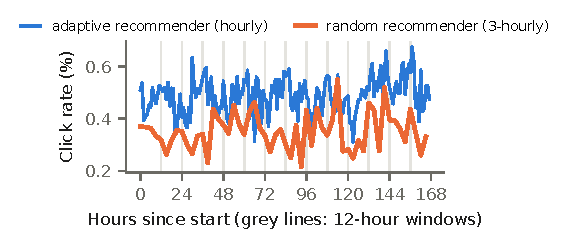
\includegraphics[width=0.75\textwidth]{figures/hourly_drift.pdf}

\raggedright
\begin{itemize}
  \item Click rate changes within each 12-hour window (grey lines).
  \item The usual standard error treats every row as independent, so it misses this.
  \item Grouping errors by hour explains most of the gap, but not the click model's bias.
\end{itemize}
\end{frame}

\begin{frame}{Finding 2: every real decision, one campaign}
\centering
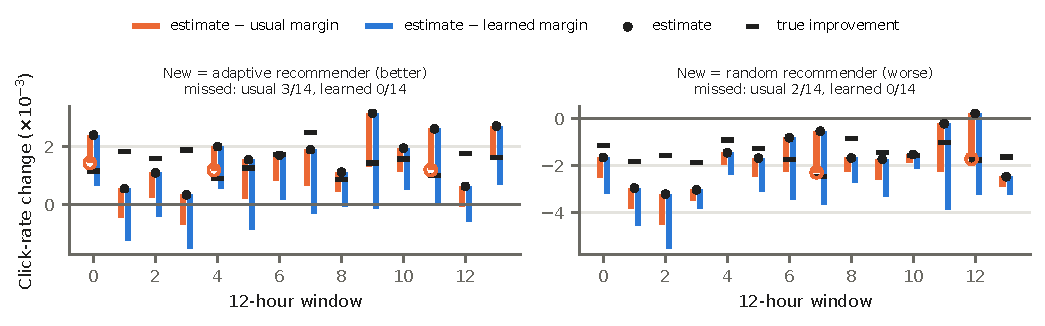
\includegraphics[width=\textwidth]{figures/decision_chart.pdf}

\raggedright
\small Bars: estimate down to estimate $-$ margin. Launch if the bar's bottom is above 0. Circle: the truth fell below the bar (a miss).
All three campaigns: usual margin misses \textcolor{warn}{\textbf{16/84}}, learned margin \textcolor{clr}{\textbf{4/84}}.
\end{frame}

\begin{frame}{Finding 2: the learned margin is safe on real data}
\begin{columns}[c]
\begin{column}{0.47\textwidth}
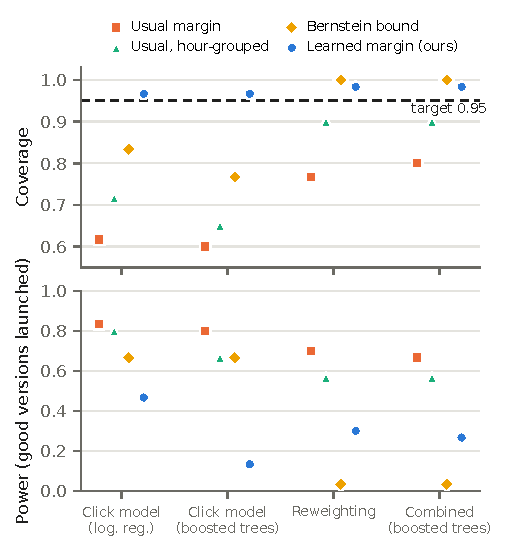
\includegraphics[width=\textwidth]{figures/obd_temporal.pdf}
\end{column}
\begin{column}{0.53\textwidth}
Each window uses only \emph{earlier} windows as history.
\begin{itemize}
  \item Usual margin: safe 60--80\%
  \item Usual, hour-grouped: 65--90\%
  \item \textcolor{clr}{\textbf{Learned margin: 95--98\%}}
  \item Bernstein bound: safe, but almost never launches
\end{itemize}
Cost: fewer launches (13--47\% vs 63--83\%). That is the price of honest uncertainty.
\end{column}
\end{columns}
\end{frame}

\begin{frame}{Finding 3: controlled experiments with exact truth}
\begin{columns}[c]
\begin{column}{0.47\textwidth}
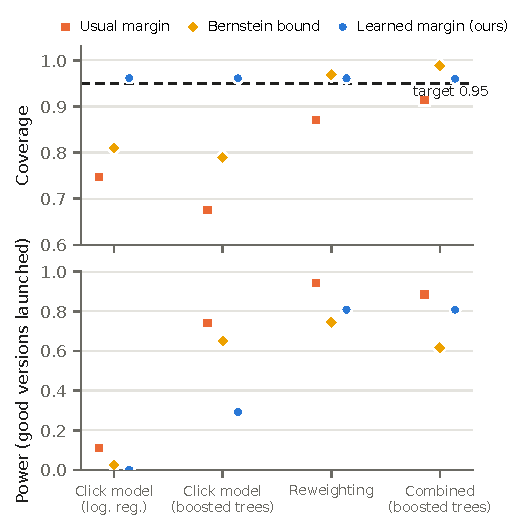
\includegraphics[width=\textwidth]{figures/semi_coverage_power.pdf}
\end{column}
\begin{column}{0.53\textwidth}
\begin{itemize}
  \item Usual margin: safe 68--91\%
  \item \textcolor{clr}{\textbf{Learned margin: 95--96\%}} for all 10 estimator variants
  \item Biased click model: wrong launches \textcolor{warn}{\textbf{27.7\%}} $\to$ \textcolor{clr}{\textbf{0\%}}
  \item History from other datasets: still 93--95\%
  \item Breaks under deliberate population shift (78--88\%), as the assumption predicts
\end{itemize}
\end{column}
\end{columns}
\end{frame}

\begin{frame}{How much history is needed?}
\begin{columns}[c]
\begin{column}{0.58\textwidth}
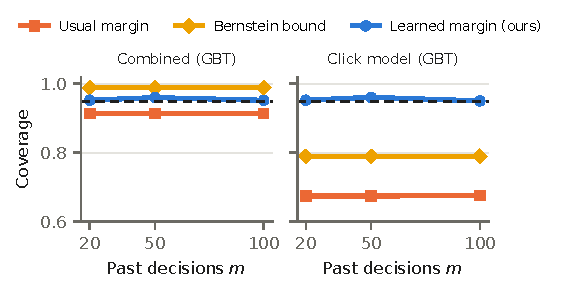
\includegraphics[width=\textwidth]{figures/coverage_vs_history.pdf}
\end{column}
\begin{column}{0.42\textwidth}
\begin{itemize}
  \item The learned margin hits the 95\% target with only \textbf{20} past decisions.
  \item More history does not change coverage; it makes the margin more stable.
  \item The usual margin stays below target however much data you have.
\end{itemize}
\end{column}
\end{columns}
\end{frame}

\begin{frame}{Adaptive margin: an ML model learns which decisions are hard}
\begin{columns}[T]
\begin{column}{0.45\textwidth}
\begin{itemize}
  \item Inputs: log size, largest/average weight, weight spread, $\log\se$
  \item \textbf{Ridge regression} or \textbf{gradient-boosted trees} predict how wrong the estimate will be
  \item Hard decisions get a bigger margin, easy ones a smaller one
\end{itemize}
\end{column}
\begin{column}{0.55\textwidth}
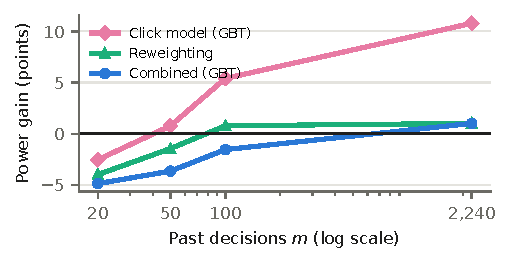
\includegraphics[width=\textwidth]{figures/adaptive_gain.pdf}

\textbf{Helps only with lots of history.} With few past decisions, the plain version is better.
\end{column}
\end{columns}
\end{frame}

\begin{frame}{Where the machine learning is}
\small
\begin{tabular}{p{0.33\textwidth}p{0.6\textwidth}}
\toprule
Model & Used for \\
\midrule
Logistic regression & Click model; the current recommender in controlled experiments; retrained versions \\
Gradient-boosted trees & Click model (stronger); difficulty model in the adaptive margin \\
Ridge regression & Difficulty model in the adaptive margin \\
Naive Bayes, $k$-NN, random forest & New recommenders in controlled experiments \\
PCA & Creates the population shift \\
Cross-fitting & Models never predict on their own training rows \\
Conformal prediction & Turns the track record into a guaranteed margin \\
\bottomrule
\end{tabular}
\vspace{0.5em}

No deep learning. No reinforcement learning: nothing learns by trial and error; we only analyse existing logs.
\end{frame}

\begin{frame}[fragile]{Live demo: the one window where the new recommender was worse}
\scriptsize
\begin{verbatim}
$ make demo
Estimated improvement in click rate: +0.00307 (standard error 0.00116)

Rule                                            est - margin  Decision
Usual margin (1.645 x se)                           +0.00116  LAUNCH
Usual margin, hour-grouped se                       +0.00054  LAUNCH
Bootstrap margin                                    +0.00120  LAUNCH
Bernstein bound                                     -0.00378  hold
Learned margin (2.73 x se, 72 past decisions)       -0.00010  hold

True improvement, measured on real traffic: -0.00035
  -> new recommender is NOT better
\end{verbatim}
\normalsize
The usual margins launch a worse recommender. The learned margin holds.
\end{frame}

\begin{frame}{Conclusion and limitations}
\begin{itemize}
  \item Offline launch decisions are only as safe as their margin.
  \item On real logs the usual margin was about \textbf{2$\times$ too small} (hourly drift + click-model bias).
  \item Learning the margin from past decisions gave the promised 95\% safety on real and controlled data.
\end{itemize}
\vspace{0.5em}
\textbf{Limitations:} needs a history of past decisions; assumes the future resembles the past; fewer launches; real data has only two recommenders.\\[0.3em]
\textbf{Next:} weight past decisions by similarity; combine with hour-grouped standard errors.
\end{frame}

\begin{frame}{Backup: what is new compared with prior work}
\small
\begin{tabular}{p{0.35\textwidth}p{0.58\textwidth}}
\toprule
Prior work & Difference \\
\midrule
Choosing the best estimator (2023--24) & We make the \emph{decision} safe for any estimator \\
High-confidence bounds (2015) & Valid only if the estimator is unbiased \\
Conformal intervals for single outcomes (2022) & We calibrate launch decisions using past decisions \\
Offline A/B testing (2018) & Uses only within-log variability \\
\bottomrule
\end{tabular}
\end{frame}

\end{document}
